\chapter{Il web ad oggi}
\section{Perché ottimizzare la propria interfaccia web?}
Le tecnologie per la produzione di applicazioni web si sono evolute esponenzialmente da quando il web era ancora un progetto pensato per scambiare documentazione scientifica in modalità elettronica. Oggi il web viene utilizzato per gli scopi più disparati, dal promuovere il proprio business a offrire veri e propri servizi ad alto traffico e scalabilità.
Molte compagnie basano il proprio business esclusivamente sul mondo web, si pensi ad un sito ecommerce o a piattaforme di condivisione come i social, Chi invece gestisce business esterni sfrutta il web e le piattaforme sviluppate su di esso per promuovere la propria attività, in un contesto diventato ormai essenziale per ogni tipo di business.
\newline
Pensiamoci, qual'è  la prima cosa che facciamo quando necessitiamo di informazioni su un particolare prodotto o servizio? oppure abbiamo bisogno di riempire un vuoto informativo in maniera tempestiva?  interroghiamo l'oracolo del nuovo millennio Google in cerca di risposte.
\newline
Il mondo web si è espanso cosi tanto da diventare un qualcosa di normale e scontato nella nostra vita quotidiana e con tante realtà che ormai spostano le loro vetrine e i loro contenuti informativi su questa tecnologia, e offrono user experience sempre più avanzate, gli utenti sono diventati sempre più esigenti in termini di performance e tempi di risposta da parte di questi servizi.Secondo uno studio condotto nel 2018 da Google, la probabilita che un utente abbandoni il sito aumenta in maniera esponenziale in base al tempo di caricamento delle pagine.\cite{mobile-page-speed}
\newline
\begin{figure}[H]
\centering
   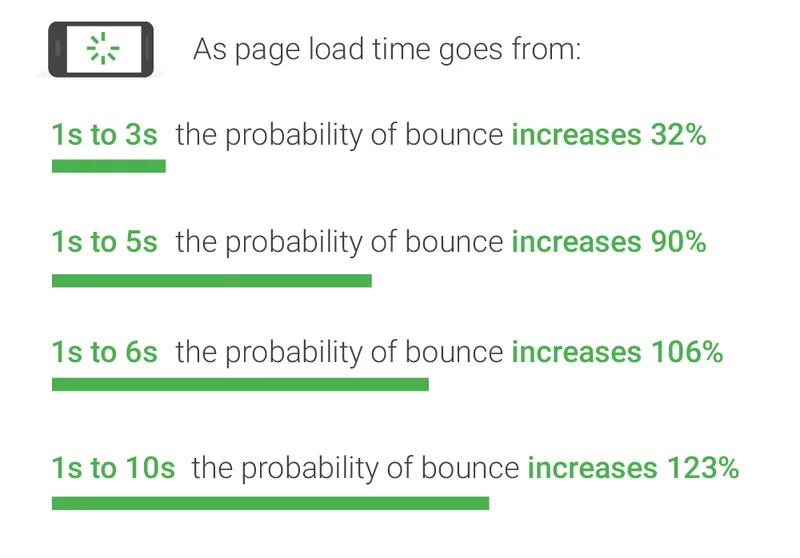
\includegraphics[scale=0.5]{resources/mobile-page-speed-new-industry.png}
\cite{mobile-page-speed}
\caption{probabilità di abbandono del sito in relazione al tempo di caricamento}
\end{figure}
Inoltre, più della metà delle richieste effettuate a questi servizi avviene da device mobile e per il 70\% dei siti analizzati i tempi di caricamento ammontano a più di 5 secondi. \cite{mobile-page-speed}

\section{Il web in numeri: statistiche}
Se si da uno sguardo alle statistiche ci si può accorgere che la maggior parte dei siti non dedica le giuste attenzioni all'ottimizzazione del proprio servizio, in particolare secondo uno studio effettuato da tooltester.com:
\begin{itemize}
    \item Il tempo di caricamento medio delle pagine è di 2.5 secondi per i device desktop e 8 per i device mobile.
    \item Il delay del primo contatto con l'utente è di 12.73 millisecondi per i device desktop e di 59.73 per i device mobile
    \item Le pagine  impiegano un tempo medio di caricamento superiore del 70.9\% su device mobile rispetto che su device desktop
    \item Gli utenti di device mobile sono al primo posto nella classifica di abbandono delle pagine con una percentuale di 56.8\% 
    \item il settore delle scienze possiede il rateo di abbandono più alto con una percentuale di 66.37\%
    \item Di tutte le tipologie di device (desktop/tablet/mobile) il tablet è quello con il minor numero di sessioni all'anno con una percentuale di 2.3%
\end{itemize}
\begin{figure}[H]
   \centering
   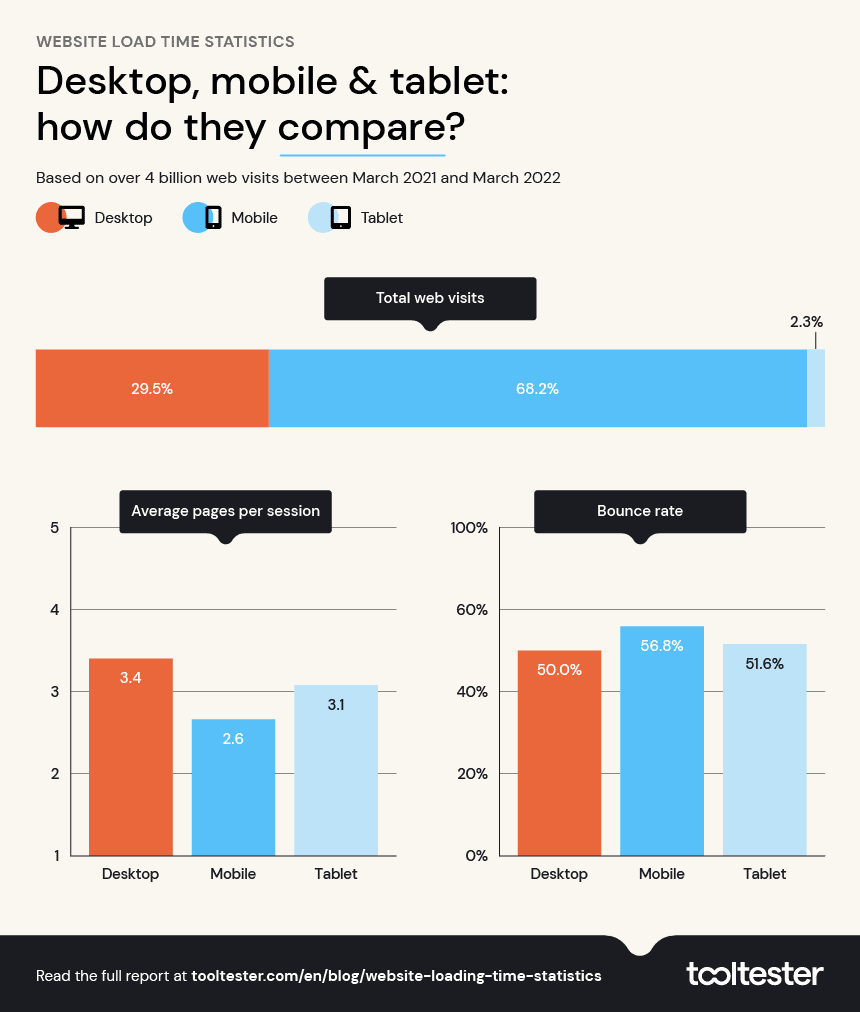
\includegraphics[scale=0.25]{resources/website-load-time-statistics-desktop-mobile-tablet.png}
\cite{website-loading-time-statistics}
\caption{Statistiche di visualizzazione pagine web}
\end{figure}


   \section{Perché Angular?}
Date queste premesse l'elaborato si pone come obbiettivo quello di mostrare le funzionalità di ottimizzazione delle performance che il framework angular offre agli sviluppatori.
\newline
Nato nel 2016 come evoluzione di angularjs e mantenuta da un team indipendente di sviluppatori google, la libreria viene ormai adottata sia per lo sviluppo di single page application ad alte prestazioni sia per la costruzione di frontend web.
\newline
La libreria offre molte possibilità agli sviluppatori
\begin{itemize}
    \item La possibilita di fare testing realtime dell'applicazione
    \item Alte prestazioni offerte dal meccanismo di change detection
    \item Alta flessibilità e scalabilità delle applicazioni
\end{itemize}
La libreria viene inoltre utilizzata da molte grandi realtà quali IBM Samsung e Paypal
\newline
\begin{figure}[H]
   \centering
   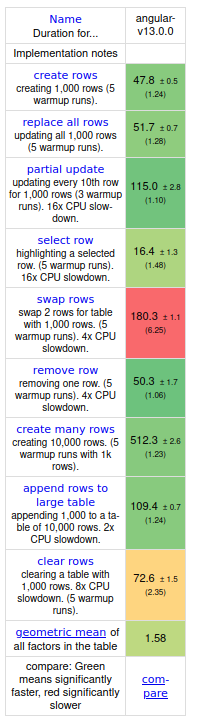
\includegraphics[scale=0.4]{resources/angular-performance.png}
\caption{test prestazioni libreria angular}
\end{figure}
